\documentclass{article}

\usepackage{iclr2027_conference,times}
\usepackage[utf8]{inputenc}
\usepackage[T1]{fontenc}
\usepackage{microtype}
\usepackage{amsmath,amssymb}
\usepackage{booktabs}
\usepackage{tabularx}
\usepackage{graphicx}
\usepackage{tikz}
\usepackage{enumitem}
\usepackage{xcolor}
\usepackage{xurl}
\usepackage{seqsplit}
\usepackage{hyperref}
\usepackage[capitalise,noabbrev]{cleveref}
\usetikzlibrary{arrows.meta,positioning}

\definecolor{FBBlue}{HTML}{1769AA}
\definecolor{FBGold}{HTML}{B77A08}
\definecolor{FBTeal}{HTML}{168C7A}
\definecolor{FBRed}{HTML}{B44743}
\definecolor{FBCharcoal}{HTML}{262B33}
\definecolor{FBPaper}{HTML}{F4F6F7}
\hypersetup{
  colorlinks=true,
  linkcolor=FBBlue,
  citecolor=FBBlue,
  urlcolor=FBBlue,
  pdftitle={FlavourBench: Executable Culinary Reward Maps for Language Model Evaluation and Post-Training},
  pdfauthor={Anonymous Authors},
  pdfsubject={Executable reward maps for evaluating culinary decisions by language models},
  pdfkeywords={language models, executable benchmarks, reward models, culinary reasoning,
    uncertainty quantification}
}
\setlist{leftmargin=*,nosep}

\newcommand{\system}{\textsc{FlavourBench}}
\newcommand{\epicure}{\textsc{Epicure}}
\newcommand{\sha}[1]{\texttt{\seqsplit{#1}}}
\newcommand{\FBModels}{27}
\newcommand{\FBTasks}{534}
\newcommand{\FBTasksPerFamily}{178}
\newcommand{\FBTasksPerPanelFamily}{89}
\newcommand{\FBPanelCount}{2}
\newcommand{\FBFamilies}{3}
\newcommand{\FBUniqueAnchors}{534}
\newcommand{\FBSelectionsPerTask}{56}
\newcommand{\FBPrefrozenScores}{29904}
\newcommand{\FBPrimaryCells}{14418}
\newcommand{\FBPairs}{351}
\newcommand{\FBSignificantPairs}{101}
\newcommand{\FBBootstrapResamples}{50000}
\newcommand{\FBPermutationResamples}{100000}
\newcommand{\FBTopModel}{Grok 4.6}
\newcommand{\FBTopScore}{65.1}
\newcommand{\FBTopCILow}{61.0}
\newcommand{\FBTopCIHigh}{69.2}
\newcommand{\FBTopGroup}{1}
\newcommand{\FBDefinitiveTop}{no}
\newcommand{\FBPanelPearson}{0.89}
\newcommand{\FBPanelSpearman}{0.80}
\newcommand{\FBIndependentClusters}{534}
\newcommand{\FBCompleteCells}{14418}
\newcommand{\FBPlanDigest}{2ba71c793c8d}

% Generated by build_stability_assets.py; do not edit.
\newcommand{\FBStabilityReplicates}{5,000}
\newcommand{\FBGeneralizability}{0.936}
\newcommand{\FBTasksForGNinety}{329}
\newcommand{\FBHalfTaskCount}{270}
\newcommand{\FBHalfRankMedian}{0.952}
\newcommand{\FBHalfRankLow}{0.897}
\newcommand{\FBHalfRankHigh}{0.980}
\newcommand{\FBHalfTopOne}{46.1\%}
\newcommand{\FBHalfTopFive}{80\%}
\newcommand{\FBStabilityArtifact}{4b359ac51db465c7a3f49fb5567a624b1ce3ad6280d309f31545e17ff2797026}

% Generated by build_selection_robustness_assets.py; do not edit.
\newcommand{\FBLOOModel}{Claude Fable 5}
\newcommand{\FBLOOOverlap}{71.0\%}
\newcommand{\FBLOORankRho}{0.955}
\newcommand{\FBLOOPairAgreement}{92.9\%}
\newcommand{\FBLOOMeanShift}{0.65}
\newcommand{\FBLOOMaxShift}{1.37}
\newcommand{\FBSelectionMaxSMD}{0.27}
\newcommand{\FBMetricMinRho}{0.938}
\newcommand{\FBMetricMinAgreement}{89.2\%}
\newcommand{\FBWeightGridPoints}{696}
\newcommand{\FBWeightMinRho}{0.980}
\newcommand{\FBWeightMedianRho}{0.991}
\newcommand{\FBRobustnessArtifact}{09ebe388b99d6da629c5ec8f8ee837ec0b01b9361f337649228602187ab44293}

% Generated by build_public_scorer_sensitivity_assets.py; do not edit.
\newcommand{\FBPublicScorerMinRho}{0.903}
\newcommand{\FBPublicScorerMaxRho}{0.957}
\newcommand{\FBPublicScorerMinPair}{86.9\%}
\newcommand{\FBPublicScorerMaxPair}{91.7\%}
\newcommand{\FBPublicScorerReplicates}{20,000}
\newcommand{\FBPublicScorerArtifact}{799550a10f13786ef356f069295d3c73ec34d5e0e8ad1394ce838af6622e5f49}

% Auto-generated by build_external_substitution_validation_assets.py.
\newcommand{\FBExternalSubRawTest}{10,747}
\newcommand{\FBExternalSubMappedEvents}{3,282}
\newcommand{\FBExternalSubPairs}{1,469}
\newcommand{\FBExternalSubNovelPairs}{594}
\newcommand{\FBExternalSubSources}{357}
\newcommand{\FBExternalSubBestLabel}{Epicure-Cooc}
\newcommand{\FBExternalSubBestPercentile}{80.6\%}

% Auto-generated by build_reward_transfer_assets.py.
\newcommand{\FBTransferPrimaryTasks}{84}
\newcommand{\FBTransferPublicTasks}{534}
\newcommand{\FBTransferPrimaryChance}{30.85}
\newcommand{\FBTransferPublicChance}{31.20}
\newcommand{\FBTransferPrimaryBase}{29.99}
\newcommand{\FBTransferPrimaryControl}{30.90}
\newcommand{\FBTransferPrimaryTreatment}{44.20}
\newcommand{\FBTransferPrimaryBaseParse}{89.29}
\newcommand{\FBTransferPrimaryControlParse}{100.00}
\newcommand{\FBTransferPrimaryTreatmentParse}{100.00}
\newcommand{\FBTransferPrimaryGain}{13.30}
\newcommand{\FBTransferPrimaryCILow}{6.52}
\newcommand{\FBTransferPrimaryCIHigh}{20.29}
\newcommand{\FBTransferPrimaryP}{1.70\!\times\!10^{-4}}
\newcommand{\FBTransferPrimaryControlBaseGain}{0.90}
\newcommand{\FBTransferPrimaryControlBaseCILow}{-4.91}
\newcommand{\FBTransferPrimaryControlBaseCIHigh}{6.85}
\newcommand{\FBTransferPrimaryControlBaseP}{0.790}
\newcommand{\FBTransferPublicBase}{28.56}
\newcommand{\FBTransferPublicControl}{31.60}
\newcommand{\FBTransferPublicTreatment}{43.33}
\newcommand{\FBTransferPublicBaseParse}{89.14}
\newcommand{\FBTransferPublicControlParse}{100.00}
\newcommand{\FBTransferPublicTreatmentParse}{100.00}
\newcommand{\FBTransferPublicGain}{11.73}
\newcommand{\FBTransferPublicCILow}{8.98}
\newcommand{\FBTransferPublicCIHigh}{14.54}
\newcommand{\FBTransferPublicP}{1.00\!\times\!10^{-5}}
\newcommand{\FBTransferPublicControlBaseGain}{3.05}
\newcommand{\FBTransferPublicControlBaseCILow}{0.46}
\newcommand{\FBTransferPublicControlBaseCIHigh}{5.68}
\newcommand{\FBTransferPublicControlBaseP}{0.021}


\title{\system{}: Executable Culinary Reward Maps for Language Model Evaluation\\
and Post-Training}
\author{Anonymous Authors}

% Leave \iclrfinalcopy commented for double-blind review.
%\iclrfinalcopy

\begin{document}
\maketitle

\begin{abstract}
Open-ended language-model evaluation often substitutes another model or a small preference panel
for a missing answer key. We introduce \system{}, which instead compiles dense answer maps from a
versioned culinary environment. Each task asks for a three-ingredient portfolio from eight
candidates; before inference, \epicure{} scores all 56 portfolios. We evaluate \FBModels{} frontier
endpoints on the same \FBTasks{} substitution, pairing, and constraint tasks, yielding
\FBCompleteCells{} complete model--task observations. Anchor-cluster bootstraps and
multiplicity-controlled paired tests resolve \FBSignificantPairs{} of \FBPairs{} model contrasts.
\FBTopModel{} has the largest point estimate (\FBTopScore{}), but the corrected evidence does not
identify a unique best endpoint. The ranking replicates across independently compiled panels and
remains similar under alternative metrics, task filters, family weights, and three public
\epicure{} checkpoints. We then run a preregistered, three-seed post-training study. LoRA SFT of a
pinned Qwen3-0.6B checkpoint on 270 \epicure{}-optimal answers improves its score on
\FBTransferPrimaryTasks{} anchor-disjoint maps by \FBTransferPrimaryGain{} points over a format-
and label-matched control (95\% CI \FBTransferPrimaryCILow{}--\FBTransferPrimaryCIHigh{},
$p=\FBTransferPrimaryP{}$), and the effect replicates on all \FBTransferPublicTasks{} public maps.
The replication gain is \FBTransferPublicGain{} points (95\% CI
\FBTransferPublicCILow{}--\FBTransferPublicCIHigh{}). On the primary split, both trained arms parse
every response while the format control does not improve on the base model. The release contains
prompts, exhaustive reward maps, raw responses, training and
evaluation manifests, statistical plans, code, and an offline verifier.
\end{abstract}

\section{Introduction}

An executable evaluator gives a benchmark a stable object to measure. Programs can be tested,
database states inspected, and games scored. Many open-ended language tasks lack that structure:
human votes are costly, model judges inherit model-dependent biases, and exact-match keys collapse
plausible answers into a binary outcome \citep{zheng2023judging,chiang2024chatbotarena}. The result
may be scalable without being auditable.

\system{} creates executable evaluation for culinary decisions. It starts from \epicure{}, a
versioned representation of 1,790 ingredients in a 300-dimensional space
\citep{radzikowski2026structure,radzikowski2026geometry}. A compiler turns substitution, pairing,
and constrained-composition operations into three-of-eight selection problems. It then enumerates
all $\binom{8}{3}=56$ legal portfolios and records a continuous reward map before any evaluated
model is called. Scoring is a deterministic lookup, not a post-hoc interpretation of generated
text.

This construction does not make \epicure{} ``correct'' in a universal culinary sense. The primary
score measures agreement with one released reward function under one published task distribution.
The benchmark is useful only if that estimand is explicit and its dependence on the reward map can
be tested. We therefore combine a complete common-task design with panel replication, clustered
inference, roster and metric sensitivity, rescoring under three public checkpoints, and an external
substitution check.

Our contributions are:
\begin{enumerate}[label=\arabic*.]
  \item an executable benchmark that freezes \FBPrefrozenScores{} graded portfolio rewards before
  model execution and exposes a single 0--100 score;
  \item a rectangular \FBModels{}-by-\FBTasks{} frontier evaluation with simultaneous uncertainty,
  all \FBPairs{} paired contrasts, and score-blind common-core construction;
  \item post-collection tests of panel, task-filter, score-definition, family-weight, and reward-map
  dependence, plus label-independent validation against observed substitutions; and
  \item a preregistered three-seed study showing that \epicure{}-optimal SFT transfers to unseen
  reward maps beyond answer-format learning, with a public-map replication and content-addressed
  training evidence.
\end{enumerate}

\begin{figure}[t]
  \centering
  \resizebox{\linewidth}{!}{%
  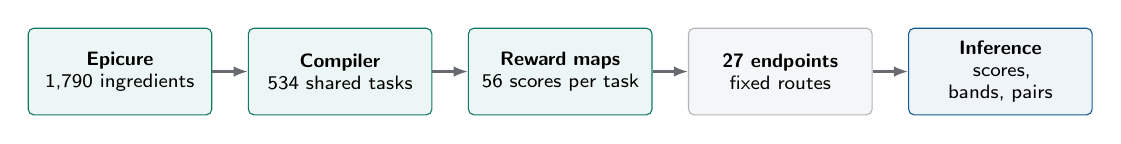
\begin{tikzpicture}[
    font=\sffamily\scriptsize,
    node distance=0.45cm,
    block/.style={draw=FBCharcoal!35,fill=FBPaper,rounded corners=2pt,
      minimum height=1.1cm,text width=2.05cm,align=center,inner sep=4pt},
    oracle/.style={block,draw=FBTeal!85!black,fill=FBTeal!8},
    result/.style={block,draw=FBBlue!85!black,fill=FBBlue!7},
    arrow/.style={-{Latex[length=1.8mm]},thick,draw=FBCharcoal!70}
  ]
    \node[oracle] (runtime) {\textbf{Epicure}\\1,790 ingredients};
    \node[oracle,right=of runtime] (compiler) {\textbf{Compiler}\\534 shared tasks};
    \node[oracle,right=of compiler] (maps) {\textbf{Reward maps}\\56 scores per task};
    \node[block,right=of maps] (models) {\textbf{27 endpoints}\\fixed routes};
    \node[result,right=of models] (release) {\textbf{Inference}\\scores, bands, pairs};
    \draw[arrow] (runtime) -- (compiler);
    \draw[arrow] (compiler) -- (maps);
    \draw[arrow] (maps) -- (models);
    \draw[arrow] (models) -- (release);
  \end{tikzpicture}}
  \caption{\system{} freezes the tasks, every candidate reward, and the inference contract before
  model execution. Evaluated models neither access \epicure{} nor judge one another.}
  \label{fig:architecture}
\end{figure}

\section{Executable benchmark construction}
\label{sec:benchmark}

\subsection{Reference environment and task families}

The primary task maps bind one exact \epicure{} data bundle and application build by content hash.
Its original training seed and source revision were not recovered, so we treat it as a fixed
reference function rather than independently established culinary ground truth. Changing the
artifact creates a new benchmark identity. Section~\ref{sec:validity} evaluates three independently
published, immutable sibling checkpoints.

For task $t$, let $\mathcal{A}_t$ be the 56 three-item subsets of its eight candidates and
$u_t(a)$ the environment utility of portfolio $a$. Invalid portfolios under a dietary or processing
constraint receive zero; valid utilities are normalized within task:
\begin{equation}
 s_t(a)=100\,\frac{u_t(a)-\min_{b\in\mathcal{A}_t}u_t(b)}
 {\max_{b\in\mathcal{A}_t}u_t(b)-\min_{b\in\mathcal{A}_t}u_t(b)}.
 \label{eq:task-score}
\end{equation}
Each task has a unique 100-point optimum. Its exact chance value is the mean of its 56 frozen
scores, not a generic percentage.

The ranked set contains \FBTasks{} tasks, balanced across two independently compiled panels and
three decision families (\cref{tab:families}). The panels have disjoint task identifiers; tasks
sharing an anchor ingredient form one cluster for inference. Candidate labels and order follow a
task-derived hash. No evaluated model proposes candidates, distractors, or scores.

\begin{table}[t]
  \caption{Complete-core task families. Each contains \FBTasksPerFamily{} tasks and uses the same
  three-of-eight response contract.}
  \label{tab:families}
  \centering
  \small
  \setlength{\tabcolsep}{4pt}
  \begin{tabularx}{\linewidth}{@{}l X X@{}}
    \toprule
    Family & Decision & Environment utility \\
    \midrule
    Substitution & Replace an anchor with a coherent three-item portfolio &
      $0.8$ anchor similarity $+0.2$ portfolio coherence \\
    Pairing & Choose three ingredients to accompany an anchor &
      $0.65$ anchor affinity $+0.35$ portfolio coherence \\
    Constraints & Choose a portfolio satisfying diet and processing limits &
      $0.7$ anchor similarity $+0.3$ coherence; invalid sets score zero \\
    \bottomrule
  \end{tabularx}
\end{table}

Prompts end with an exact \texttt{FINAL\_SELECTION} marker and require three distinct labels. The
parser reads the final marker line, sorts the labels as an unordered set, and performs one reward-map
lookup; free-form explanation does not affect the score. Missing markers, duplicate labels,
provider failures, and abnormal finishes remain in the execution ledger but cannot enter the
shared core.

The score maps are graded rather than exact keys with 55 equivalent mistakes. Substitution and
pairing tasks each have 56 distinct scores at the median, exact chance means of 45.2 and 45.0, and
median top-two gaps of 5.6 points. Constraint maps are deliberately sparse: infeasible portfolios
score zero, producing an exact chance mean of 3.4 and a median top-two gap of 37.3. The examples in
\cref{tab:examples} show why partial credit matters: non-optimal portfolios can be far apart even
when both satisfy the response syntax.

\begin{table}[t]
  \caption{Deterministically selected common-core examples. Parentheses give the frozen task score;
  the supplement includes complete prompts, choices, score maps, and raw responses.}
  \label{tab:examples}
  \centering
  \scriptsize
  \begin{tabularx}{\linewidth}{@{}l X X X@{}}
\toprule
Family & Prompt & Higher-ranked selection & Lower-ranked selection \\
\midrule
Substitution & Select three alternatives to `boursin cheese` that best preserve its dairy role, regional context, and mutual portfolio coherence. & caciocavallo, fromage blanc, grana padano (100) & fromage blanc, quail egg, goose egg (15) \\
Pairing & Select the three-ingredient bundle with the strongest learned pairing to `sweetbread` and the best internal coherence. & parsnip, cipollini onion, porcini mushroom (92) & parsnip, pickled onion, peppadew pepper (0) \\
Constraints & For a dish centered on `potato`, select three vegetarian complements with NOVA processing level at most 2; among valid portfolios, maximize learned pairing and coherence. & parsley, black pepper, thyme (100) & cheese, bay leaf, parsley (0) \\
\bottomrule
\end{tabularx}

\end{table}

\subsection{Primary score}

For model $m$, panel $p$, family $f$, and selected task set $T_{pf}$, let $Y_{mt}$ be the frozen
portfolio score. The primary metric is
\begin{equation}
 F_m=\frac{1}{6}\sum_{p=1}^{2}\sum_{f=1}^{3}
      \frac{1}{|T_{pf}|}\sum_{t\in T_{pf}}Y_{mt}.
 \label{eq:fb-score}
\end{equation}
Because all six strata contain \FBTasksPerPanelFamily{} tasks, this equals the ordinary mean over
the \FBTasks{} cells. Every ranked endpoint has one valid response for every selected task. Failures
are not assigned a culinary score and are not dropped model by model; task eligibility is determined
jointly from status and parser validity before any selected portfolio or score is loaded.

\section{Evaluation and inference}
\label{sec:design}

\subsection{Endpoint panel and common core}

The panel covers 27 endpoints from 16 laboratories: OpenAI, Anthropic, Google, xAI, Meta, Kimi,
Qwen, Z.ai, DeepSeek, ByteDance, Thinking Machines, MiniMax, NVIDIA, Mistral, Tencent, and Cohere.
It includes multiple endpoints from several laboratories to separate lab-level branding from
endpoint-level behavior. The manifest binds requested and returned identities, model version,
provider route, supported controls, completion contract, and collection block. Automatic fallback
is disabled. When transport validation required a route change, the complete model block was rerun;
successful cells from superseded blocks were never pooled. Exact endpoints and routes are listed in
Appendix~\ref{app:routes}.

Each panel compiler creates 160 candidates per family. Within every panel--family stratum, the
analysis selects the first \FBTasksPerPanelFamily{} tasks eligible for all 27 endpoints under a fixed
SHA-256 order. Selection code sees only response status and parser validity until task identifiers
are fixed. The result is a rectangular \FBModels{}-by-\FBTasks{} matrix rather than a leaderboard in
which models answer different task subsets.

\subsection{Uncertainty, multiplicity, and stability}

The content-addressed analysis plan fixes all inferential choices. We draw
\FBBootstrapResamples{} bootstrap samples over the \FBUniqueAnchors{} anchor clusters, keeping tasks
that share an anchor together, and report both pointwise score intervals and a simultaneous max-$t$
band over all 27 scores. Every pair of endpoints is compared on the same 534 tasks using a two-sided
anchor-cluster sign-flip test with \FBPermutationResamples{} Monte Carlo draws; Holm correction
controls familywise error across all \FBPairs{} comparisons. A separate Holm family tests each
endpoint against the exact taskwise random-portfolio mean. Bootstrap rank intervals and contiguous
non-rejection groups accompany point ranks.

Two diagnostics ask whether 534 tasks are enough. First, family--panel-stratified subsets of 30,
60, 90, 150, and 270 tasks are drawn without replacement \FBStabilityReplicates{} times and compared
with the full point order. Second, a crossed model-by-task variance decomposition estimates a
descriptive generalizability coefficient for relative endpoint decisions. Neither calculation turns
these fixed tasks or endpoints into random samples from an unspecified population.

We also rerun task selection after omitting each endpoint; compare selected with unselected compiler
candidates; recompute ranks with chance-adjusted gain, action percentile, and exact-optimum rate; and
enumerate all one-percentage-point family weights from 0.20 to 0.50. These are retrospective
sensitivity analyses, not additional confirmatory rankings.

\section{Results}
\label{sec:results}

\subsection{Leaderboard and resolved comparisons}

\FBTopModel{} has the largest point estimate, \FBTopScore{}, with simultaneous 95\% interval
[\FBTopCILow{}, \FBTopCIHigh{}] (\cref{fig:leaderboard}). Of the \FBPairs{} prespecified pairwise
contrasts, \FBSignificantPairs{} survive Holm correction. The upper ranks therefore form an
unresolved group: the experiment supports many broad differences, but not a unique best endpoint.
Every point in the figure is computed from the identical 534-task core.

\begin{figure}[t]
  \centering
  
\includegraphics[width=0.98\linewidth]{figures/complete-core-leaderboard-forest.pdf}
  \caption{FlavourBench Score and simultaneous 95\% max-$t$ intervals. Group numbers summarize the
  multiplicity-controlled pairwise graph; point ranks inside a group are not established total
  orders. Exact values and rank intervals appear in Appendix~\ref{app:leaderboard}.}
  \label{fig:leaderboard}
\end{figure}

\subsection{Replication and design sensitivity}

The two panel-specific score vectors correlate at Pearson $r=\FBPanelPearson{}$ and rank
$\rho=\FBPanelSpearman{}$. The crossed-design relative-decision generalizability coefficient is
\FBGeneralizability{}; the same variance model estimates \FBTasksForGNinety{} balanced tasks for
0.90. At \FBHalfTaskCount{} tasks, the median rank correlation with the full point order is
\FBHalfRankMedian{} (empirical 95\% range \FBHalfRankLow{}--\FBHalfRankHigh{}), yet the full point
leader survives only \FBHalfTopOne{} of draws. This distinction matters: the global score is stable
while the identity of a single winner is not.

Omitting the endpoint that most constrained eligibility and reapplying the frozen task hash retains
\FBLOOOverlap{} of tasks; among the remaining models, rank correlation is \FBLOORankRho{} and the
largest score shift is \FBLOOMaxShift{} points. None of 42 comparisons between selected and
unselected task candidates survives Holm correction, and the largest standardized difference is
\FBSelectionMaxSMD{}. Alternative score definitions retain rank correlations of at least
\FBMetricMinRho{}; across \FBWeightGridPoints{} moderate family-weight settings, the minimum is
\FBWeightMinRho{}. The point leader alternates between Grok 4.6 and Gemini 3.1 Pro, again arguing
against a definitive winner claim.

\begin{figure}[t]
  \centering
  
\includegraphics[width=0.58\linewidth]{figures/complete-core-panel-replication.pdf}
  \par\vspace{0.3em}
  
\includegraphics[width=\linewidth]{figures/complete-core-task-count-stability.pdf}
  \caption{Top: independent-panel scores for all endpoints. Bottom: stability of score-blind task
  subsets relative to the complete 534-task point order. Panel agreement and subset stability
  support the global score; leader preservation shows why the top point estimate is not definitive.}
  \label{fig:replication-stability}
\end{figure}

\begin{table}[t]
  \caption{Compact robustness summary. Rank statistics compare with the complete primary point
  order; these diagnostics do not redefine the confirmatory score.}
  \label{tab:robustness}
  \centering
  \small
  \begin{tabularx}{\linewidth}{@{}X l X@{}}
    \toprule
    Diagnostic & Result & Reading \\
    \midrule
    Independent panels & $r=.89$, $\rho=.80$ & broad replication \\
    Crossed-design coefficient & $G=.936$ & high relative-score reliability \\
    Half-size subsets & median $\rho=.952$ & stable order, unstable winner \\
    Leave-one-endpoint task filter & $\rho=.955$ & limited roster dependence \\
    Alternative score definitions & $\rho\geq.938$ & broad metric robustness \\
    Moderate family weights & $\rho\geq.980$ & little weight dependence \\
    Public reward checkpoints & $\rho=.903$--$.957$ & broad reward-map robustness \\
    \bottomrule
  \end{tabularx}
\end{table}

\section{Reward-map and construct validity}
\label{sec:validity}

\subsection{Replacing the reward map}

The primary runtime is reproducible by hash but lacks a recovered training lineage. We therefore
rescore all \FBCompleteCells{} fixed model decisions with Epicure-Cooc, Epicure-Core, and
Epicure-Chem at immutable public revisions \citep{radzikowski2026geometry}. This post-hoc analysis
does not call any endpoint again. Median within-task rank correlation between the primary and
replacement 56-action maps is 0.660--0.752; exact optima agree on 27.7\%--38.4\% of tasks. Despite
that local change, aggregate model-rank correlations are \FBPublicScorerMinRho{}--
\FBPublicScorerMaxRho{} and \FBPublicScorerMinPair{}--\FBPublicScorerMaxPair{} of pair directions
agree. The same sampled point leader appears under both maps in only 38.9\%--53.8\% of bootstrap
draws, supporting broad order rather than a fixed winner.

\begin{figure}[t]
  \centering
  
\includegraphics[width=\linewidth]{figures/complete-core-public-scorer-sensitivity.pdf}
  \caption{Reward-map sensitivity with prompts and model decisions held fixed. Left: rank
  trajectories for the primary top ten. Right: aggregate rank and pair-direction agreement with
  the primary map.}
  \label{fig:public-scorer}
\end{figure}

\subsection{Observed substitutions}

Recipe1MSubs derives standardized substitutions from recipe-user comments
\citep{fatemi2023substitute}. A hash-bound protocol, fixed before checkpoint scores were inspected,
uses exact ingredient-token matches, deduplicates directed source--target pairs, and ranks each
observed target by source--candidate cosine similarity. The primary candidate set is restricted to
the target's existing food group so that broad category recognition cannot clear the null. Pair
percentiles are averaged within source and then equally across sources; 50,000 source-cluster
bootstrap draws form intervals, with Holm correction across three checkpoint tests.

Exact matching yields \FBExternalSubPairs{} unique directed test pairs over
\FBExternalSubSources{} sources (\cref{tab:external}). All three intervals exclude the 0.5 chance
percentile after Holm correction ($p_{\mathrm{Holm}}<10^{-4}$). The result persists on
\FBExternalSubNovelPairs{} pairs absent from Recipe1MSubs training. These labels are external to
\epicure{} fitting, but Recipe1MSubs and part of \epicure{} share Recipe1M ancestry. The test is
therefore label-independent convergent validation, not corpus-independent validation, and it does
not validate the unrecovered primary runtime directly.

\begin{table}[t]
  \caption{Observed-substitution validation. Percentile is the equal-source rank against
  same-food-group candidates; ``novel'' retains pairs absent from Recipe1MSubs training.}
  \label{tab:external}
  \centering
  \small
  \begin{tabular}{lccc}
\toprule
Checkpoint & Percentile [95\% CI] & Novel pairs & Hit@10 \\
\midrule
Cooc & 0.806 [0.788, 0.824] & 0.754 & 0.133 \\
Core & 0.800 [0.781, 0.819] & 0.735 & 0.172 \\
Chem & 0.780 [0.761, 0.798] & 0.718 & 0.155 \\
\bottomrule
\end{tabular}

\end{table}

\begin{figure}[t]
  \centering
  
\includegraphics[width=\linewidth]{figures/complete-core-external-substitution-validation.pdf}
  \caption{Observed targets ranked against same-food-group alternatives. Filled points use all
  mapped test pairs; open points retain only directed pairs absent from Recipe1MSubs training.}
  \label{fig:external-substitution}
\end{figure}

\section{Culinary profiles}

The aggregate score does not collapse the three decision families into the same behavior
(\cref{fig:families}). Gemini 3.1 Pro has the highest substitution mean, Kimi K3 the highest pairing
mean, and Grok 4.6 the highest constraint mean; no endpoint leads every family. These values should
be read within family rather than as a difficulty ordering because the frozen chance surfaces differ
substantially. The decomposition is nevertheless useful diagnostically: a lab can distinguish a
model that retrieves plausible substitutes from one that composes coherent bundles or reliably
respects feasibility constraints.

\section{Reward transfer beyond format learning}
\label{sec:training}

The exhaustive maps can supervise a policy as well as score one. We test the narrow claim that
\epicure{} supervision transfers to unseen maps beyond learning the required response syntax. The
protocol and analysis code were public before optimization outcomes were generated. It pins
Qwen3-0.6B at one repository revision \citep{yang2025qwen3}, partitions 270 training, 72 validation,
and 84 primary-transfer tasks by disjoint ingredient anchor, and reserves the 534 leaderboard maps
for a secondary replication. Candidate sets and prompt hashes are also disjoint across the lab
splits.

Three seeds receive three epochs of all-linear LoRA SFT \citep{hu2022lora} with rank 16, effective
batch size 16, learning rate $10^{-4}$, completion-only loss, and the final checkpoint without
validation-based selection. The treatment completion is each task's \epicure{} optimum. The control
rotates those same A--H portfolios onto different prompts within family and panel, preserving every
prompt, row count, completion length, and portfolio-label histogram while preventing accidental
optima. Greedy decoding and a 64-token limit are fixed for every arm. Unparseable completions remain
in the score at zero.

The preregistered estimand is the equal-family treatment-minus-control score difference. A
50,000-draw crossed bootstrap resamples matched training seeds and anchors within the six
family--panel strata; a two-sided 100,000-draw sign-flip test operates on anchor effects averaged
over seeds. The interval therefore includes empirical seed and anchor variation, whereas the
$p$-value tests held-out-anchor effects conditional on the three realized seed pairs; it is not a
population-level test over retraining randomness. The protocol defines three points as a
practically material gain. There is one primary contrast, so it receives no multiplicity
adjustment.

\begin{table}[t]
  \caption{Reward transfer. Scores average three training seeds except the unmodified base.
  $\Delta$ is Epicure SFT minus format control; the public-map row is a declared secondary
  replication opened only after the primary analysis was sealed.}
  \label{tab:transfer}
  \centering
  \scriptsize
  \resizebox{\linewidth}{!}{% Auto-generated by build_reward_transfer_assets.py.
\begin{tabular}{@{}lrrrrr@{}}
\toprule
Evaluation & Base & Format control & Epicure SFT & $\Delta$ [95\% CI] & $p$ \\
\midrule
Anchor-disjoint transfer ($n=84$) & 29.99 & 30.90 & 44.20 & +13.30 [6.52, 20.29] & $1.70\!\times\!10^{-4}$ \\
Public-map replication ($n=534$) & 28.56 & 31.60 & 43.33 & +11.73 [8.98, 14.54] & $1.00\!\times\!10^{-5}$ \\
\bottomrule
\end{tabular}
}
\end{table}

On the \FBTransferPrimaryTasks{} anchor-disjoint tasks, \epicure{} SFT scores
\FBTransferPrimaryTreatment{} versus \FBTransferPrimaryControl{} for the format control, a
\FBTransferPrimaryGain{}-point gain (95\% CI
\FBTransferPrimaryCILow{}--\FBTransferPrimaryCIHigh{}, $p=\FBTransferPrimaryP{}$). All three
primary seed effects are positive. Both trained arms parse \FBTransferPrimaryControlParse{}\% of responses;
the base parses \FBTransferPrimaryBaseParse{}\%. Format training alone changes the base score by
only \FBTransferPrimaryControlBaseGain{} points (95\% CI
\FBTransferPrimaryControlBaseCILow{}--\FBTransferPrimaryControlBaseCIHigh{},
$p=\FBTransferPrimaryControlBaseP{}$). The public-map replication yields a
\FBTransferPublicGain{}-point effect (95\% CI
\FBTransferPublicCILow{}--\FBTransferPublicCIHigh{}, $p=\FBTransferPublicP{}$;
\cref{fig:transfer}); all three replication seed effects are positive. Appendix~\ref{app:transfer}
reports every seed and the descriptive family decomposition.

The control is empirically consequential. On the public maps it improves on the base by
\FBTransferPublicControlBaseGain{} points (95\% CI
\FBTransferPublicControlBaseCILow{}--\FBTransferPublicControlBaseCIHigh{},
$p=\FBTransferPublicControlBaseP{}$), consistent with removing parse failures. A treatment--base
comparison would fold that syntax gain into the reward effect. Treatment--control differences are
positive in all six evaluation-by-family cells and largest for constraints in both evaluations;
these family rows are descriptive rather than separately tested.

\begin{figure}[t]
  \centering
  
\includegraphics[width=\linewidth]{figures/complete-core-reward-transfer.pdf}
  \caption{Held-out scores and matched treatment effects. Small points are training seeds;
  connecting lines pair the control and treatment initialized with the same seed. The right panel
  reports the prespecified crossed-bootstrap interval. The dashed line marks the three-point
  practical threshold, not a null hypothesis.}
  \label{fig:transfer}
\end{figure}

These results isolate learning of this released reward function from answer-format learning. They
do not establish human preference, cooked-food quality, general capability, reinforcement-learning
improvement, or transfer outside the culinary environment.

\section{Related work}

General evaluation includes broad suites such as HELM \citep{liang2022helm}, difficult knowledge
tests such as MMLU-Pro and GPQA \citep{wang2024mmlupro,rein2023gpqa}, contamination-resistant sets
\citep{white2024livebench,jain2024livecodebench}, and human-preference arenas
\citep{chiang2024chatbotarena}. BetterBench emphasizes explicit benchmark documentation and
validity claims \citep{reuel2024betterbench}. Executable benchmarks replace preference inference
with observable outcomes: SWE-bench runs repository tests \citep{jimenez2023swebench}, BFCL checks
function calls \citep{patil2025bfcl}, and $\tau$-bench inspects database state
\citep{yao2024taubench}. \system{} applies the same principle to a dense domain reward surface.
RewardBench instead evaluates learned reward models on chosen--rejected pairs
\citep{lambert2024rewardbench}. Our reward source is a versioned program rather than a learned
preference model, and the transfer experiment tests whether its supervision changes unseen-task
decisions after controlling for answer syntax.

Culinary resources cover ingredient networks, recipes, substitutions, planning, nutrition, and
food knowledge \citep{ahn2011flavor,garg2018flavordb,salvador2017recipe1m,
fatemi2023substitute,choi2024cookingsense,wu2025recipe2plan,hua2025nutribench,
eftimov2026foodbench,jin2026diningbench}. Our contribution is narrower: paired frontier-model
measurement against an exhaustive culinary decision environment, rather than recipe generation or
factual question answering.

\section{Limitations}

FlavourBench Score is agreement with a released reward map, not universal taste. Public-checkpoint
rescoring and Recipe1MSubs provide convergent evidence, but do not validate the primary runtime's
unrecovered training lineage, pairing and constraint rewards, sensory preference, or cooked
outcomes. Within-task min--max normalization creates an interpretable 0--100 scale while discarding
absolute utility magnitudes. The tasks test constrained ingredient selection, not full recipes,
safety advice, embodied cooking, or long-horizon kitchen planning.

The complete-core rule removes model-specific missingness but changes the estimand to tasks every
endpoint completed; roster sensitivity cannot rule out unrecorded selection effects. Results bind
specific model versions, providers, routes, and collection dates. The dense maps make reward-based
learning possible, but the transfer evidence comes from LoRA SFT of one 0.6B checkpoint over three
seeds. It does not compare training algorithms or model scales. The public replication reuses the
same trained adapters on new maps and therefore strengthens task transfer, not independent training
replication.

\section{Conclusion}

\system{} evaluates open-ended culinary decisions without asking one language model to grade
another. Exhaustive reward maps make partial credit deterministic; a rectangular common-task
design makes comparisons paired; simultaneous intervals and corrected tests distinguish broad
performance differences from an unsupported winner narrative. In a controlled post-training
study, supervision from those maps changes decisions on unseen anchors beyond what format-matched
SFT explains. The public artifacts reconstruct every reported score, contrast, training run, table,
and figure.

\clearpage
\subsection*{AI use statement}

Generative AI tools assisted with methodology feedback, implementation, data cleaning and
formatting, statistical-analysis support, interpretation, literature discovery, figure production,
and drafting and editing the manuscript. They did not originate the empirical observations: model
responses and benchmark records are retained as content-addressed artifacts, and quantitative
claims are regenerated by tested analysis code. The authors reviewed the AI-assisted work;
citations were checked against source records, release verifiers check the numerical artifacts, and
the authors take responsibility for the final content.

\subsection*{Ethics statement}

No human participants were recruited. The external check uses an existing public research dataset;
the release records its provenance and hashes and redistributes only aggregate validation outputs,
not the raw Recipe1MSubs files. The benchmark measures a bounded culinary construct and should not
be interpreted as nutrition, allergy, food-safety, or medical advice. Provider credentials and
private communications are excluded from the release.

\subsection*{Reproducibility statement}

The anonymous supplement contains the exact task maps, model and route manifest, raw selected
responses, completion records, frozen analysis plans, public-checkpoint score maps, aggregate
external-validation artifact, deterministic asset builders, and an offline verifier. It also
contains the reward-transfer protocol, training data, raw held-out generations, run manifests,
analysis code, commands, and environment contract needed to reconstruct the leaderboard,
statistical tables, and vector figures without provider access. Appendices report execution routes,
protocol constants, per-family scores, and robustness analyses.

\bibliography{references}
\bibliographystyle{iclr2027_conference}

\clearpage
\appendix

\section{Complete leaderboard}
\label{app:leaderboard}

\begin{table}[h]
  \caption{Complete leaderboard on the common 534-task core. Rank intervals use the anchor-cluster
  bootstrap; groups summarize the Holm-controlled pairwise graph.}
  \centering
  \scriptsize
  \resizebox{\linewidth}{!}{\begin{tabular}{@{}r l r c c c@{}}
\toprule
Rank & Model & FB Score & simultaneous 95\% CI & rank 95\% CI & group \\
\midrule
1 & Grok 4.6 & 65.1 & [61.0, 69.2] & [1, 5] & 1 \\
2 & Gemini 3.1 Pro & 65.0 & [60.8, 69.1] & [1, 6] & 1 \\
3 & GPT-5.6 Sol Pro & 64.2 & [60.1, 68.4] & [1, 8] & 1 \\
4 & Muse Spark 1.2 & 63.8 & [59.6, 67.9] & [1, 10] & 1 \\
5 & GPT-5.6 Terra Pro & 63.7 & [59.5, 67.8] & [1, 11] & 1 \\
6 & Claude Fable 5 & 63.4 & [59.2, 67.5] & [2, 13] & 1 \\
7 & GPT-5.6 Luna Pro & 62.6 & [58.5, 66.8] & [4, 14] & 1 \\
8 & Claude Opus 5 & 62.5 & [58.4, 66.6] & [3, 15] & 1 \\
9 & Qwen3.8 A95B & 62.1 & [57.9, 66.2] & [4, 17] & 1 \\
10 & Kimi K3 & 62.1 & [57.9, 66.2] & [5, 16] & 1 \\
11 & Gemini 3.6 Flash & 62.0 & [57.7, 66.2] & [4, 17] & 1 \\
12 & DeepSeek V4 Pro 0813 & 62.0 & [57.8, 66.1] & [5, 17] & 1 \\
13 & Qwen 3.8 Max & 61.5 & [57.4, 65.6] & [7, 18] & 1 \\
14 & Tencent HY 3 & 61.5 & [57.3, 65.7] & [6, 19] & 1 \\
15 & MiniMax M3 & 60.9 & [56.8, 65.1] & [8, 20] & 1 \\
16 & GLM 5.3 & 60.6 & [56.4, 64.8] & [8, 20] & 1 \\
17 & Muse Glimmer 30B & 59.9 & [55.9, 63.9] & [12, 21] & 2 \\
18 & Seed 2.1 Turbo & 59.7 & [55.4, 64.0] & [12, 22] & 2 \\
19 & Inkling & 59.6 & [55.4, 63.8] & [12, 22] & 2 \\
20 & Claude Sonnet 5 & 59.5 & [55.4, 63.7] & [13, 22] & 2 \\
21 & GLM 5.2 & 58.5 & [54.2, 62.7] & [16, 23] & 2 \\
22 & Nemotron 3.5 Lightning & 57.4 & [53.2, 61.6] & [19, 25] & 2 \\
23 & Command A & 56.7 & [52.5, 60.9] & [20, 25] & 2 \\
24 & DeepSeek V4 Flash & 55.4 & [51.1, 59.7] & [22, 26] & 2 \\
25 & Mistral Large 3 & 55.4 & [51.4, 59.5] & [22, 26] & 2 \\
26 & Llama 4 Maverick & 53.7 & [49.6, 57.7] & [24, 26] & 3 \\
27 & Command R+ & 47.9 & [43.7, 52.0] & [27, 27] & 3 \\
\bottomrule
\end{tabular}
}
\end{table}

\section{Exact execution routes}
\label{app:routes}

\begin{table}[h]
  \caption{Frozen execution routes. Automatic fallback is disabled; route changes represent
  complete model-block replacements, never cell pooling.}
  \centering
  \scriptsize
  \resizebox{\linewidth}{!}{\begin{tabular}{@{}l l l l@{}}
\toprule
Model & Backend & Panel 1 route & Panel 2 route \\
\midrule
Grok 4.6 & openrouter & xai/zdr & xai/zdr \\
Gemini 3.1 Pro & openrouter & google-ai-studio & google-ai-studio \\
GPT-5.6 Sol Pro & openrouter & openai/flex & openai/flex \\
Muse Spark 1.2 & openrouter & meta & meta \\
GPT-5.6 Terra Pro & openrouter & openai/flex & openai/flex \\
Claude Fable 5 & openrouter & google-vertex/global & google-vertex/global \\
GPT-5.6 Luna Pro & openrouter & openai/flex & openai \\
Claude Opus 5 & openrouter & azure/us & azure/us \\
Qwen3.8 A95B & openrouter & alibaba & alibaba \\
Kimi K3 & openrouter & morph & morph \\
Gemini 3.6 Flash & openrouter & google-vertex/us & google-vertex/us \\
DeepSeek V4 Pro 0813 & openrouter & gmicloud/fp8 & gmicloud/fp8 \\
Qwen 3.8 Max & openrouter & alibaba & alibaba \\
Tencent HY 3 & openrouter & gmicloud/bf16 & gmicloud/bf16 \\
MiniMax M3 & openrouter & venice/fp8 & venice/fp8 \\
GLM 5.3 & zai\_coding\_direct & zai-coding-plan-direct & zai-coding-plan-direct \\
Muse Glimmer 30B & openrouter & fireworks & fireworks \\
Seed 2.1 Turbo & openrouter & seed/fp8 & seed/fp8 \\
Inkling & openrouter & deepinfra/fp8 & deepinfra/fp8 \\
Claude Sonnet 5 & openrouter & amazon-bedrock/claude-on-aws & amazon-bedrock/claude-on-aws \\
GLM 5.2 & openrouter & coreweave/fp4 & coreweave/fp4 \\
Nemotron 3.5 Lightning & openrouter & venice/fp4 & venice/fp4 \\
Command A & openrouter & cohere & cohere \\
DeepSeek V4 Flash & openrouter & deepinfra/fp4 & deepinfra/fp8 \\
Mistral Large 3 & openrouter & mistral & mistral \\
Llama 4 Maverick & openrouter & digitalocean & digitalocean \\
Command R+ & openrouter & cohere & cohere \\
\bottomrule
\end{tabular}
}
\end{table}

\section{Task-map and protocol diagnostics}

\begin{table}[h]
  \caption{Frozen task-map diagnostics. Chance is the uniform mean over all 56 portfolios; top gap
  is the median best--second-best score difference.}
  \centering
  \small
  \begin{tabular}{@{}l r r r@{}}
\toprule
Family & Exact chance & Top gap & Distinct scores \\
\midrule
Substitution & 45.2 & 5.6 & 56 \\
Pairing & 45.0 & 5.6 & 56 \\
Constraints & 3.4 & 37.3 & 4 \\
\bottomrule
\end{tabular}

\end{table}

\begin{table}[h]
  \caption{Primary design and inference constants.}
  \centering
  \small
  \begin{tabular}{@{}l r@{}}
    \toprule
    Quantity & Frozen value \\
    \midrule
    Models & \FBModels{} \\
    Panels / families & 2 / 3 \\
    Tasks per model & \FBTasks{} \\
    Unique anchor clusters & \FBUniqueAnchors{} \\
    Portfolios per task & \FBSelectionsPerTask{} \\
    Complete cells & \FBCompleteCells{} \\
    Bootstrap replicates & \FBBootstrapResamples{} \\
    Sign-flip replicates & \FBPermutationResamples{} \\
    Pairwise hypotheses & \FBPairs{} \\
    Common-core rule & status/parser only; score-blind \\
    \bottomrule
  \end{tabular}
\end{table}

\section{Per-family scores}

\begin{table}[h]
  \caption{Mean score by family. Every row uses identical tasks.}
  \centering
  \scriptsize
  \resizebox{0.86\linewidth}{!}{\begin{tabular}{@{}l r r r@{}}
\toprule
Model & Substitution & Pairing & Constraints \\
\midrule
Grok 4.6 & 66.1 & 70.9 & 58.2 \\
Gemini 3.1 Pro & 69.0 & 71.6 & 54.2 \\
GPT-5.6 Sol Pro & 66.2 & 72.5 & 54.1 \\
Muse Spark 1.2 & 65.9 & 70.3 & 55.0 \\
GPT-5.6 Terra Pro & 66.1 & 72.1 & 52.8 \\
Claude Fable 5 & 68.2 & 70.6 & 51.3 \\
GPT-5.6 Luna Pro & 64.5 & 69.7 & 53.7 \\
Claude Opus 5 & 67.2 & 69.9 & 50.4 \\
Qwen3.8 A95B & 66.0 & 67.8 & 52.5 \\
Kimi K3 & 65.5 & 73.7 & 47.0 \\
Gemini 3.6 Flash & 68.1 & 66.2 & 51.6 \\
DeepSeek V4 Pro 0813 & 66.4 & 69.5 & 49.9 \\
Qwen 3.8 Max & 66.6 & 68.5 & 49.5 \\
Tencent HY 3 & 66.0 & 67.9 & 50.5 \\
MiniMax M3 & 65.4 & 69.9 & 47.6 \\
GLM 5.3 & 63.7 & 69.6 & 48.4 \\
Muse Glimmer 30B & 65.1 & 66.8 & 47.8 \\
Seed 2.1 Turbo & 65.3 & 66.2 & 47.6 \\
Inkling & 63.6 & 65.8 & 49.5 \\
Claude Sonnet 5 & 65.3 & 69.2 & 44.1 \\
GLM 5.2 & 63.6 & 67.2 & 44.5 \\
Nemotron 3.5 Lightning & 65.3 & 64.3 & 42.5 \\
Command A & 64.7 & 63.9 & 41.6 \\
DeepSeek V4 Flash & 63.1 & 63.2 & 40.1 \\
Mistral Large 3 & 60.4 & 65.8 & 40.0 \\
Llama 4 Maverick & 59.4 & 61.4 & 40.2 \\
Command R+ & 56.7 & 54.9 & 32.0 \\
\bottomrule
\end{tabular}
}
\end{table}

\section{Selection and metric sensitivity}
\label{app:robustness}

\begin{figure}[h]
  \centering
  
\includegraphics[width=\linewidth]{figures/complete-core-selection-robustness.pdf}
  \caption{Left: task overlap after omitting each endpoint and rerunning frozen selection. Right:
  agreement between the primary metric and alternative summaries.}
\end{figure}

\begin{table}[h]
  \caption{Alternative summaries of the same 534 decisions.}
  \centering
  \small
  \begin{tabular}{@{}l r r l@{}}
\toprule
Score summary & Rank $\rho$ & Pair order & Point leader \\
\midrule
FlavourBench Score & 1.000 & 100.0\% & Grok 4.6 \\
Chance-adjusted gain & 0.985 & 96.0\% & Gemini 3.1 Pro Preview \\
Action percentile & 0.969 & 93.4\% & Grok 4.6 \\
Exact-optimum rate & 0.938 & 89.2\% & Grok 4.6 \\
\bottomrule
\end{tabular}

\end{table}

\section{Public-checkpoint sensitivity}

\begin{figure}[h]
  \centering
  
\includegraphics[width=\linewidth]{figures/complete-core-public-scorer-sensitivity.pdf}
  \caption{Rank trajectories and aggregate agreement after replacing the reward map while holding
  all tasks and model selections fixed.}
\end{figure}

\begin{table}[h]
  \caption{Aggregate agreement with the primary reward map.}
  \centering
  \small
  \begin{tabular}{@{}l r r r l@{}}
\toprule
Reward map & Task-map $\rho$ & Model-rank $\rho$ & Pair order & Point leader \\
\midrule
Epicure-Cooc & 0.752 & 0.957 & 91.7\% & Grok 4.6 \\
Epicure-Core & 0.672 & 0.915 & 88.0\% & Grok 4.6 \\
Epicure-Chem & 0.660 & 0.903 & 86.9\% & Grok 4.6 \\
\bottomrule
\end{tabular}

\end{table}

\section{External substitution validation}

\begin{figure}[h]
  \centering
  
\includegraphics[width=\linewidth]{figures/complete-core-external-substitution-validation.pdf}
  \caption{Observed Recipe1MSubs targets ranked against same-food-group alternatives. Filled
  points use all mapped test pairs; open points retain only pairs absent from the training split.}
\end{figure}

\section{Reward-transfer protocol and diagnostics}
\label{app:transfer}

\begin{table}[h]
  \caption{Frozen reward-transfer protocol. Validation loss is monitored but never selects a
  checkpoint.}
  \centering
  \small
  \begin{tabular}{@{}l l@{}}
    \toprule
    Component & Frozen value \\
    \midrule
    Base & Qwen3-0.6B, revision \texttt{c1899de289a04d1}\ldots \\
    Conditions & unmodified base; format-control SFT; Epicure-optimum SFT \\
    Train / validation / transfer & 270 / 72 / 84 anchor-disjoint tasks \\
    Training seeds & 20260824, 20260825, 20260826 \\
    LoRA & rank 16; alpha 32; dropout .05; all linear layers \\
    Optimization & 3 epochs; AdamW; LR $10^{-4}$; effective batch 16 \\
    Checkpoint rule & final adapter only; no validation selection \\
    Decoding & greedy; thinking disabled; 64 new tokens \\
    Primary score & equal family and panel; unparseable responses score zero \\
    Inference & 50,000 crossed bootstraps; 100,000 anchor sign flips \\
    \bottomrule
  \end{tabular}
\end{table}

\begin{table}[h]
  \caption{Descriptive reward-transfer scores by task family. $\Delta$ is Epicure SFT minus
  format control; these family rows were not separate confirmatory hypotheses.}
  \centering
  \small
  % Auto-generated by build_reward_transfer_assets.py.
\begin{tabular}{@{}llrrrr@{}}
\toprule
Evaluation & Family & Base & Format control & Epicure SFT & $\Delta$ \\
\midrule
Transfer & Substitution & 57.93 & 41.62 & 52.79 & +11.16 \\
Transfer & Pairing & 28.66 & 46.34 & 53.56 & +7.23 \\
Transfer & Constraint & 3.39 & 4.73 & 26.24 & +21.51 \\
\midrule
Public & Substitution & 47.63 & 47.43 & 52.39 & +4.96 \\
Public & Pairing & 34.36 & 43.59 & 53.62 & +10.02 \\
Public & Constraint & 3.69 & 3.78 & 23.99 & +20.21 \\
\bottomrule
\end{tabular}

\end{table}

\begin{table}[h]
  \caption{Matched training-seed scores. Each $\Delta$ compares adapters initialized with the
  same seed.}
  \centering
  \small
  % Auto-generated by build_reward_transfer_assets.py.
\begin{tabular}{@{}lrrrrrr@{}}
\toprule
& \multicolumn{3}{c}{Anchor-disjoint transfer} & \multicolumn{3}{c}{Public-map replication} \\
\cmidrule(lr){2-4}\cmidrule(l){5-7}
Seed & Control & Epicure & $\Delta$ & Control & Epicure & $\Delta$ \\
\midrule
20260824 & 31.61 & 44.47 & +12.86 & 32.06 & 44.74 & +12.69 \\
20260825 & 31.19 & 44.53 & +13.34 & 31.10 & 42.40 & +11.30 \\
20260826 & 29.89 & 43.59 & +13.70 & 31.65 & 42.85 & +11.20 \\
\bottomrule
\end{tabular}

\end{table}

\section{Panel, task-count, pairwise, and family diagnostics}

\begin{figure}[h]
  \centering
  
\includegraphics[width=0.78\linewidth]{figures/complete-core-panel-replication.pdf}
  \caption{Independent-panel scores for all 27 endpoints.}
\end{figure}

\begin{figure}[h]
  \centering
  
\includegraphics[width=\linewidth]{figures/complete-core-task-count-stability.pdf}
  \caption{Stability of score-blind task subsets relative to the complete point order.}
\end{figure}

\begin{figure}[h]
  \centering
  
\includegraphics[width=0.88\linewidth]{figures/complete-core-pairwise-matrix.pdf}
  \caption{All paired endpoint contrasts after Holm correction. Grey cells are unresolved.}
\end{figure}

\begin{figure}[h]
  \centering
  
\includegraphics[width=0.88\linewidth]{figures/complete-core-family-heatmap.pdf}
  \caption{Mean score by culinary decision family. Each column contains 178 identical tasks per
  endpoint; the primary score gives the three families equal weight.}
  \label{fig:families}
\end{figure}

\begin{figure}[h]
  \centering
  
\includegraphics[width=0.88\linewidth]{figures/complete-core-rank-intervals.pdf}
  \caption{Point ranks and 95\% bootstrap rank intervals.}
\end{figure}

\end{document}
